\begin{surferPage}[Sextica de Barth]{A S\^extica de  Barth}
    Esta superf\'icie de grau $6$ (s\^extica) foi constru\'ida por Wolf Barth em 1996.
    
   A S\^extica de  Barth tem ao todo $65$ singularidades.
%    (wenn man die $15$ im Bild nicht sichtbaren, ``unendlich fernen'', mitz�hlt)%
   Este \'e o n\'umero m\'aximo poss\'ivel de singularidades numa s\^extica como mostraram Jaffe e Ruberman logo ap\'os a constru\c c\~ao de Barth --- portanto, o recorde mundial de Barth
    \'e imbat\'ivel!


    A constru\c c\~ao de Barth foi uma grande surpresa porque durante muito tempo  pensou-se que as superf\'icies de grau $6$ s\'o podiam ter $64$ singularidades.

   Uma caracter\'istica marcante da constru\c c\~ao \'e a sua simetria icosa\'edrica;
    a figura mostra um icosaedro e os seus planos de simetria:  
%    Die Abb.\ zeigt diesen platonischen K�rper und seine Symmetrie - Ebenen: 
%    und diese Ebenen gemeinsam mit der Barth Sextik in einem Bild.     
    % 
  \begin{center}
      \vspace*{-0.1cm}
      \begin{tabular}{@{}c@{\ \ }c@{\,}c@{}}
        \begin{tabular}{@{}c}
          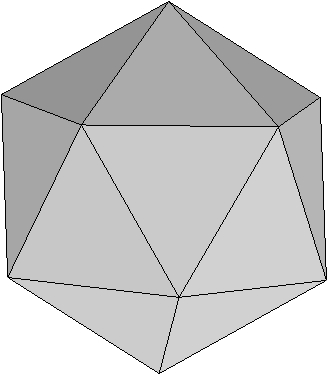
\includegraphics[width=1.4cm]{./../../common/images/icosah}
        \end{tabular}
        &
        \begin{tabular}{@{}c}
          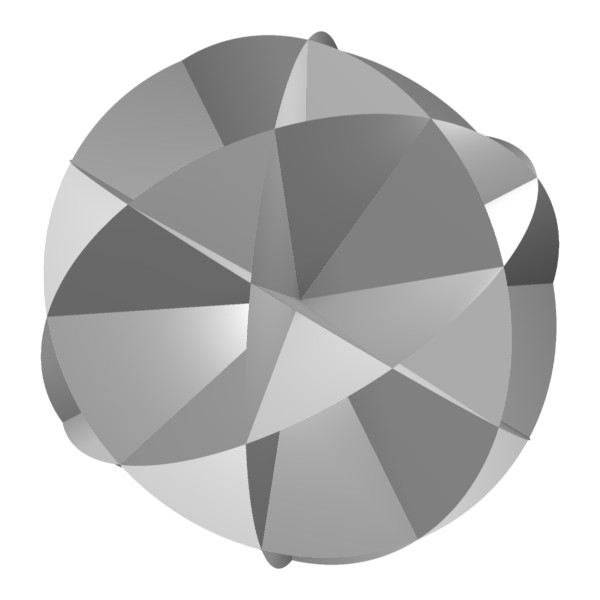
\includegraphics[width=1.4cm]{./../../common/images/barth_sextic_planes}
        \end{tabular}
        &
        \begin{tabular}{c@{}}
          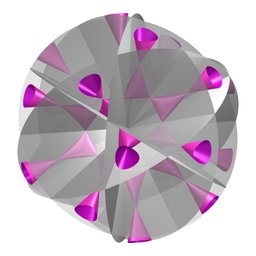
\includegraphics[width=1.4cm]{./../../common/images/barth_sextic_and_planes}
        \end{tabular}
      \end{tabular}
    \end{center}
    \vspace*{-0.1cm}

    A S\^extica de  Barth satisfaz a equa\c c\~ao
    $P_6 - \alpha K^2=0,$ onde $P_6$
   representa os 
    seis planos de simetria, $K=x^2+y^2+z^2-1$ \'e a esfera unit\'aria e
    $\alpha=\frac{1}{4}(2+\sqrt{5})$.
\end{surferPage}
